\documentclass{beamer}
\usepackage{tikz}
\usepackage{pgfplots}
\pgfplotsset{compat=1.18}

\usetheme{default}
\title{Network Flow and Architecture Topology}

\begin{document}

\begin{frame}{Overlay Node Diagrams}
  \framesubtitle{Visualizing Inter-Service Messaging via TikZ}
  \begin{center}
    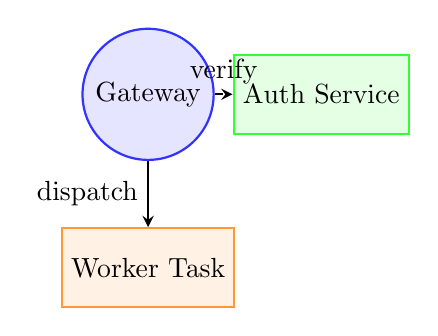
\begin{tikzpicture}[node distance=2.2cm, auto, thick]
      \node[circle, draw=blue!80, fill=blue!10, minimum size=1.2cm] (gw) {Gateway};
      \node[rectangle, draw=green!80, fill=green!10, minimum size=1.0cm, right of=gw] (auth) {Auth Service};
      \node[rectangle, draw=orange!80, fill=orange!10, minimum size=1.0cm, below of=gw] (worker) {Worker Task};

      \draw[->, >=stealth, dashed] (gw) -- node[above] {verify} (auth);
      \draw[->, >=stealth] (gw) -- node[left] {dispatch} (worker);
    \end{tikzpicture}
  \end{center}

  \begin{block}{Topology Note}
    TikZ environments encapsulate vector path primitives without breaking document parsing.
  \end{block}
\end{frame}

\end{document}
